\chapter{Stability Conditions}\label{chap:stabilities}
\thispagestyle{empty}
\def\semi{\angle\!}
\newcommand{\thin}{\asymp}
\def\cab{\CC_{[a,b)}}
\def\R{\mathbb{R}}
\def\eps{\varepsilon}
\def\sl{\text{\japanese{切}}}
\section{Introduction}
\epigraph{The cleanest cut is the one you withhold}{?}
The notion of \emph{Bridgeland stability}\footnote{There is an unavoidable clash of notation between stability conditions as described here,\index{Stability conditions} and the abstract notion of stability for a category. We underline here that this analogy does not exist.} comes from theoretical Physics, and was proposed by T\@. Bridgeland in order to better understand a construction in String Theory, the so\hyp{}called \emph{$\Pi$\hyp{}stability} of \cite{douglas2002dirichlet,douglas2001d}; Bridgeland showed that this notion has a natural interpretation in the language of triangulated categories (the idea of identifying objects of the derived category of sheaves on a space with physical D\hyp{}branes dates back to the work of Moore and Harvey \cite{harvey1998algebras}). 

The main result outlined in \cite{Brid,Bridge2} is that the set of all stability conditions on a given triangulated category $\cate{T}$ can be naturally endowed with a topology, induced by a generalized metric. This allows one to define interesting geometric structures out from a triangulated category.

Up to now, a great effort has been put (sometimes, unfortunately, to no avail) into explicitly describing the spaces of stability conditions attached to derived categories of certain algebraic varieties, and to study some of their geometric properties; at the moment of writing, a general theory of these spaces is missing\footnote{See \cite{Bridge2}, where the author says:
\begin{quote}
there is some yet\hyp{}to\hyp{}be discovered construction that will allow one to define interesting geometric structures on these spaces. \omissis the agreement between spaces of stability conditions and moduli spaces of conformal field theories is impressive enough to suggest that stability conditions do indeed capture some part
of the mathematics of string theory. My own feeling is that at some point in the near future the notion of a stability condition will be subsumed into some more satisfactory framework.
\end{quote}
The present chapter is a --clumsy or not, the reader will decide-- first step towards this more satisfactory framework.}

The main aim of the present chapter is to re\hyp{}enact the classical theory of \cite{Brid} in the framework of stable $\infty$\hyp{}categories. In this respect, this is one of the important chapters of the present thesis, as it constitutes one of the main applications of the language initiated by the ``Rosetta stone'' theorem \refbf{thm:rosetta}. Nevertheless, we only concentrate on a single piece of the rather vast theory of stability conditions on categories, limiting uourselves to showing that given two ``close enough'' stability functions $Z$ and $W$ and a slicing $J$ compatible with $Z$ then there exists a slicing compatible with $W$, close enough to $J$. A more detailed  recovering of other major results about the space of stability conditions will hopefully be discussed in a forthcoming article \cite{infty-stab}. Although our proof will closely follow the original argument by Bridgeland, there are a few points where the use of the language developed in the previous chapters of this thesis allow us to give a somehow neater treatment.

Bridgeland's theory exploits some notable\footnote{Peculiar to the standard topological structure of the set of real numbers, but not fully essential: see \cite{GKR} for an enlightening ``formal theory of stability functions'', which has been a constant source of inspiration for the present chapter.} properties of increasing families of $t$\hyp{}structures on a triangulated category $\CC$, indexed by the set of real numbers, \ie monotonic $\mathbb{Z}$\hyp{}equivariant functions $\mathbb R\to \textsc{ts}(\CC)$; we paved the way for this definition in our \achap \refbf{chap:hearts}.

\index{Slicing}These collections are called ($\mathbb R$\hyp{})\emph{slicings} in the stable setting; an extremely remarkable result, hidden in Bridgeland's original formulation and made clear by the torsio\hyp{}entric perspective, is the following:
\begin{quote}
simple topological properties of $\mathbb R$ (completeness as a metric space, properties of the standard euclidean topology and of the topology of lower convergence generated by the base $\{[a,b)\mid a,b\in\mathbb Q\}$\dots) reflect into categorical properties of slicings 
\end{quote}
A deeper analysis of this phenomenon occupies \S\refbf{slici}.
\begin{notat}\label{assumpts}
We make a number of blanket assumptions throughout the chapter: $\CC$ is, as always, a stable $\infty$\hyp{}category, and $\tee$ is a $t$\hyp{}structure on $\CC$; we often demand that $\CC$ is cocomplete, and $\tee$ is left, right or two\hyp{}sided complete. If $J\colon \mathbb{R}\to \ts(\CC)$ is a slicing, we define $\hrt_t=\CC_{[t,t+1)}$; the collection $\{\hrt_t\}$ is called the \emph{heart} of the slicing. The set of slicings $J\colon \R\to \fs(\CC)$ is denoted \index{.slicings@$\sl_{\R}(\CC)$} $\sl_{\R}(\CC)$\footnote{The Japanese verb {\japanese{切る}} (``kiru'', \emph{to cut}) contains the radical {\japanese{切}}, the same of \emph{katana}.}. The real line has to be thought as a time\hyp{}axis, in such a way that a slicing consists of ``a collection of cuttings at prescribed time''; the value of the slicing $J$ at time $\lambda$, $J(\lambda)  =(\CC_{\ge\lambda}, \CC_{<\lambda})$, will often be called the \emph{slice at time $\lambda$}, or the \emph{$\lambda$\hyp{}slice} of $J$. One has the inclusion $\CC_{\geq \lambda_0}\subseteq \bigcap_{\lambda <\lambda_0}\CC_{\geq \lambda}$.
A slicing will be called \emph{continuous} at $\lambda_0$ if
\[
\bigcap_{\lambda>\lambda_0}\CC_{\geq \lambda}=\CC_{\geq \lambda_0}.
\]
It will be called continuous if it is continuous at $\lambda_0$ for every $\lambda_0\in \mathbb{R}$. We also set
\[
\CC_{\leq \lambda_0}=\bigcap_{\lambda>\lambda_0}\CC_{< \lambda}.
\]
Notice that if  $\lambda_0<\lambda_1$, then $\CC_{\leq \lambda_0}\cap \CC_{\geq \lambda_1}=\{0\}$ since, by definition of $\CC_{\leq \lambda_0}$, we have $\CC_{\leq \lambda_0}\subseteq \CC_{<\lambda_1}$. Finally, for $\lambda_0\leq \lambda_1$ we set
\[
\CC_{[\lambda_0,\lambda_1]}=\CC_{\geq \lambda_0}\cap \CC_{\leq \lambda_1}.
\]
Also, as a shorthand notation, we write $\CC_{\lambda}=\CC_{[\lambda,\lambda]}$ for any $\lambda\in \mathbb{R}$.
\end{notat}
\begin{definition}
Let $\CC_0$ be a full subcategory of an stable $\infty$\hyp{}category $\CC$, and let $X$ be an object of $\CC_0$. If we have a pullout diagram 
\[
\begin{kD}
\lattice[mesh]{
\obj X_s; & \obj X; \\
\obj 0; & \obj X_q; \\	
};
\mor X_s -> X -> X_q <- 0 <- X_s;
\end{kD}
\]
in $\CC$ with $X_s$ and $X_q$ in $\CC_0$, then we say that $X_s$ is a \emph{subobject} of $X$ and that $X_q$ is a quotient of $X$ (relative to $\CC_0$).
\end{definition}
\index{Category!Artinian---}
\begin{definition}\label{artinnoether}
A full subcategory $\CC_0$ of a stable $\infty$\hyp{}category $\CC$ is called
\emph{of finite length} (or simply \emph{finite}) 
if for each object $A\in\CC_0$ there is no infinite ascending chain of subobjects of $A$ (equivalently, there is no infinite descending chain of quotients of $A$).
\end{definition}
\section{Slicings}\label{slici}
\epigraph{\japanese{疾く斬るって...剣はそんな小さなものかね}}{Kam\={\i}zumi Nobutsuna}
Let $J\colon \R\to \fs(\CC)$ be a continuous slicing.
\begin{definition}[Suprema and infima]\label{sup.n.inf}
For any object $A$ of $\CC$ we set
\begin{align*}
\sup(A) &=\inf\{\lambda\in \R: A\in \CC_{<\lambda}\};\\
\inf(A) &=\sup\{\lambda\in \R: A\in \CC_{\geq\lambda}\}
\end{align*}
with the convention $\sup(0)=-\infty$ and $\inf(0) = +\infty$ (if $\CC$ is \emph{left\fshyp{}right complete}, \cite[\abbrv{Def} \textbf{1.2.1.19}]{LurieHA}, the zero object is the only object whose $\sup$ and $\inf$ are not finite).\index{sup-e-inf@$\sup$ and $\inf$}
\end{definition}
\begin{remark}\label{rem.bounds}
It follows directly from the definition that $A\in \CC_{\geq \mu}$ implies $\inf(A)\geq \mu$ and $A\in \CC_{<\mu}$ implies $\sup(A)\leq \mu$. In particular, if $A\in \cab = \CC_{\ge a}\cap \CC_{<b}$ then $a\leq\inf(A)$ and $\sup(A) \leq b$.
\end{remark}
\begin{definition}
A continuous slicing $J$ will be called \emph{regular} if for any nonzero object $A$ in $\CC_{[a,b)}$ one has $\sup(A)<b$.
\end{definition}
Unless otherwise stated, all slicings considered in the following will be regular.
\begin{lemma}\label{lemma.maggiore.minore}
If $\inf(A)> \mu$ then $A\in \CC_{\geq \mu}$ and if $\sup(A)<\mu$ then $A\in \CC_{<\mu}$. In particular, it follows that for any $A\neq 0$ one has $\inf(A)\leq \sup(A)$ and $A\in \CC_{[\inf(A),\sup(A)]}$.
\end{lemma}
\begin{proof}
If $\inf(A)> \mu$ there exists $\lambda_\mu>\mu$ such that $A\in\CC_{\geq \lambda_\mu}$. Since $\lambda_\mu>\mu$, one immediately gets $A\in\CC_{\geq \mu}$. The proof for $\sup(A)$ is analogous. It follows from this that $A\in \bigcap_{\mu<\inf(A)}\CC_{\geq \mu}=\CC_{\geq \inf(A)}$ and $A\in \bigcap_{\mu>\sup(A)}\CC_{<\mu}=\CC_{\leq \sup(A)}$. If $A\neq 0$ this gives $\CC_{\geq \inf(A)}\cap \CC_{\leq \sup(A)}\neq \{0\}$ and so $\inf(A)\leq \sup(A)$ and $A\in\CC_{[\inf(A),\sup(A)]}$. 
\end{proof}
This proves that for a regular slicing the two inequalities $a\le \inf(A)$ and $\sup(A) < b$ for a nonzero object $A$ in $\CC_{[a,b)}$ form a chain:
\begin{corollary}\label{cor.estimates}
Let $J$ be a regular slicing and let $A\in \cab$ be a nonzero object. Then $a\leq \inf(A)\leq \sup(A) < b$.
\end{corollary}
An important result links together the contractibility of mapping spaces $\CC(X,Y)$ and suitable inequalities between infima and suprema of co\fshyp{}domains of these maps.
\begin{lemma}\label{lem.zero.morphism}
If $\inf(X)>\sup(Y)$ then $\CC(X,Y)=\{0\}$.
\end{lemma}
\begin{proof}
Let $t\in \R$ be such that $\sup(Y)<t<\inf(X)$. Then $X\in \CC_{\geq t}$ and $Y\in \CC_{<t}$, by Lemma \refbf{lemma.maggiore.minore}; the object\hyp{}orthogonality of classes in the slice at time $t$ allows us to conclude.
\end{proof}
The situation is depicted as follows: there is a ``natural direction'' in which nonzero morphisms of $(\CC,J)$ go: if $\inf(X)$ is greater than $\sup(Y)$, then $Y$ only receives zero morphisms from $X$.
\begin{center}
\begin{figure}[H]
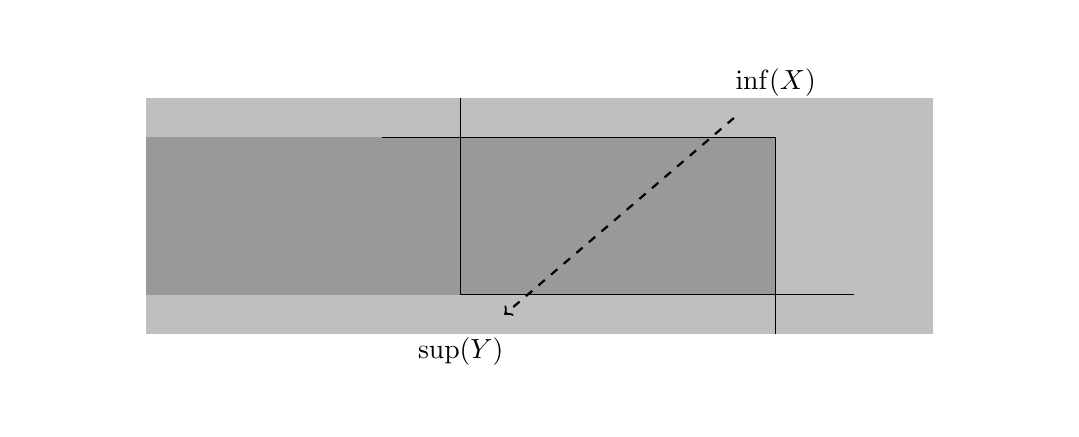
\begin{tikzpicture}
\draw[line width=3cm,lightgray] (-5,0) -- (5,0);
\draw[line width=2cm,gray!80!white] (-5,0) -- (3,0);
\draw[thin] (-2, 1) -- (3,1) -- (3,-1.5);
\draw[thin] (-1, 1.5) -- (-1, -1) -- (4, -1);
\node[circle,above] (sup) at (3,1) {$\inf(X)$};
\node[circle,below] (inf) at (-1, -1) {$\sup(Y)$};
\draw[dashed,thick,->] (sup) -- (inf);
\end{tikzpicture}
\caption{Lemma \refbf{lem.zero.morphism}.}
\end{figure}
\end{center}
Taking the contrapositive, the above Lemma gives the following.
\begin{lemma}\label{lem.opposite}
Let $f\colon X\to Y$ be a nonzero morphism in $\CC$. Then $\inf(X)\leq \sup(Y)$.
\end{lemma}
\begin{remark}
Lemma \refbf{lem.opposite} provides an additional proof of the fact that for a nonzero object $A$ in $\CC$ one has $\inf(A)\leq \sup(A)$. Indeed, if $A$ is nonzero, then $\mathrm{id}_A\colon A\to A$ is a nonzero morphism.
\end{remark}
\begin{lemma}\label{lem.exists.morphism}
Let $A$ be an object in $\CC$ and let $\mu<\sup(A)$. Then there exists a nonzero morphism $f\colon A_\mu\to A$ with $\inf(A_\mu)\geq \mu$.  Similarly, if $\mu>\inf(A)$ then there exists a nonzero morphism $f\colon A\to A_\mu$ with $\sup(A_\mu)\leq \mu$.
\end{lemma}
\begin{proof}
Since $\mu<\sup(A)$, we have $\mu\notin\{\lambda\in \R: A\in \CC_{<\lambda}\}$ and so $A\notin \CC_{<\mu} = \CC_{\geq \mu}^\perp$, and so there exists $A_\mu\in \CC_{\geq \mu}$ and a nonzero morphism $f\colon A_\mu\to A$. Since $A\in \CC_{\geq \mu}$, we have $\inf(A)\geq \mu$ by Remark \refbf{rem.bounds}. The proof of the second part of the statement is analogous. 
\end{proof}
\index{Subcategory!thin ---}
\begin{definition}[Thin subcategory]\label{thin.subcat}
The subcategories $\cab$ of a slicing show an extremely notable behaviour when $[a,b)$ is a ``sufficiently small'' interval: we call every such $\cab$ a \emph{thin} subcategory, having in mind \cite[\adef \textbf{7.2}]{Brid}; alternatively, we will call $\cab$ the $[a,b)$\hyp{}endocardium of the slicing $J$(the reason for this quaint choice of notation is explained in \S\refbf{hearts.endocar}).
\end{definition}
\begin{lemma}\label{lem:thin.are.closed}
Let  
 \[
\begin{kD}
\lattice[mesh={4em}{4em}]{
  \obj A; & \obj B; \\
  \obj 0; & \obj C; \\
};
\mor A -> B -> C;
\mor * -> 0 -> *;
\pullout{A}{C};
\end{kD}
 \]
be a fiber sequence in $\CC$ with $A,B$ and $C$ in $\cab$ with $b-a\leq 1$. Then $\sup(A)\leq \sup(B)$ and $\inf(B)\leq \inf(C)$.
\end{lemma}
\begin{proof}
We only prove $\sup(A)\leq \sup(B)$ , the other proof being dual. Assume $\sup(A)>\sup(B)$. Then there exists $\mu$ with $\sup(A)>\mu>\sup(B)$ and so by Lemma \refbf{lem.exists.morphism} there exists a nonzero morphism $f\colon A_\mu\to A$, with $\inf(A_\mu)\geq \mu>\sup(B)$. By Lemma \refbf{lem.zero.morphism}, the composition $A_\mu\xrightarrow{f} A\to B$ is zero, and so (by the universal property and the 3\hyp{}for\hyp{}2 property of pullbacks) the morphism $f$ factors through $C[-1]$. Since the composition $f\colon A_\mu\to C[-1]\to A$ is nonzero, so is the morphism $A_\mu\to C[-1]$, and so by Lemma \refbf{lem.opposite} $\sup(B)<\inf(A_\mu)\leq \sup(C[-1])=\sup(C)-1$. This gives $|\sup(B)-\sup(C)|>1$. On the other hand, since $B,C\in \cab$, by Corollary \refbf{cor.estimates}, both $\sup(B)$ and $\sup(C)$ lie in the interval $[a,b]$ and so $|\sup(B)-\sup(C)|\leq |a-b|\leq 1$.
\end{proof}
 \begin{remark}\label{good.inequalities} Lemma \refbf{lem:thin.are.closed} in particular implies that, if $b-a\leq 1$ and 
   \[
\begin{kD}
\lattice[mesh={4em}{4em}]{
  \obj A; & \obj B; \\
  \obj 0; & \obj C; \\
};
\mor A -> B -> C;
\mor * -> 0 -> *;
\pullout{A}{C};
\end{kD}
 \]
is a fiber sequence with vertices in $\mathbf{C}_{[a,b)}$ and with $B\in \mathbf{C}_{[\tilde{a},\tilde{b})}$, for some $a\leq \tilde{a}<\tilde{b}\leq b$, then $A\in \mathbf{C}_{[a,\tilde{b})}$ and $C\in \mathbf{C}_{[\tilde{a},b)}$. 
\end{remark}
We also record a direct proof of this fact, independent from \refbf{lem:thin.are.closed}. 
Since $(\CC_{<\tilde{b}},\CC_{\geq\tilde{b}})$ is a $t$\hyp{}structure on $\CC$, we have a pullout diagram
\[
\begin{kD}
\lattice[mesh]{
	\obj 0;  &  \obj (Age):A_{\geq \tilde{b}}; & \obj A;  \\
&\obj (01):0; & \obj (Ale):A_{<\tilde{b}};\\
&& \obj (02):0; \\
};
\mor 0 {e_{\tilde{b}}}:-> Age {m_{\tilde{b}}}:-> A -> Ale {m_{\tilde{b}}}:-> 02;
\mor Age -> 01 -> Ale;
\end{kD}
\]
with $A_{\geq \tilde{b}}$ in $\CC_{\geq \tilde{b}}$ and $A_{<\tilde{b}}$ in $\CC_{<\tilde{b}}$. Since $a\leq \tilde{b}$, we have $\EE_{\tilde{b}} \subseteq \EE_a$ and so $A\to A_{<\tilde{b}}$ is in $\EE_a$. Since $A\in \CC_{[a,b)}\subseteq \CC_{\geq a}$, the terminal morphism $A\to 0$ is in ${\EE_a}$. So, by the 3\hyp{}for\hyp{}2 property of ${\EE_a}$ also $A_{<\tilde{b}}\to 0$ is in $\EE_a$, i.e., $A_{<\tilde{b}}\in \CC_{\geq a}$. Therefore $A_{<\tilde{b}}\in \CC_{[a,\tilde{b})}$; we will write $A_{<\tilde{b}}=A_{[a,\tilde{b})}$ to emphasize this fact. Similarly we have $A_{\geq \tilde{b}}\in \CC_{[\tilde{b},b)}$ and we write $A_{\geq \tilde{b}}=A_{[\tilde{b},b)}$.

Consider now  the pasting of pullout diagrams
\[
\begin{kD}
\lattice[mesh]{
	& \obj C[-1]; & \obj (01):0;\\
	\obj (Abb):A_{[\tilde{b},b)}; & \obj A; & \obj B; \\
	\obj (02):0; & \obj (Aab):A_{[a,\tilde{b})}; & \obj K;\\
	&\obj 0; & \obj C; \\
};
\mor C[-1] -> 01 -> B -> K -> C;
\mor C[-1] -> A <- Abb -> 02 -> Aab -> 0 -> C;
\mor B <- A -> Aab -> K;
\end{kD}
\]
Since $A_{[\tilde{b},b)}$ is in $\CC_{[\tilde{b},b)}$ and $B\in \CC_{[\tilde{a},\tilde{b})}$, the morphism $A_{[\tilde{b},b)}\to A\to B$ is the zero morphism and so $A_{[\tilde{b},b)}\to A$ factors through $C[-1]$. But $C[-1]\in \CC_{[a-1,b-1)}$ and $b-1\leq a<\tilde{b}$, so that $\CC(A_{[\tilde{b},b)}, C[-1])=0$. 
This implies that $A_{[\tilde{b},b)}\to A$ is the zero morphism, and so $A_{[\tilde{b},b)}=0$ and $A=A_{[a,\tilde{b})}$. The proof for $C$ is dual.
\begin{remark}
If $X\in \CC_{[0,1)}\setminus \CC_{\{0\}}$, then there is a nonzero morphism $Y_\eps\to X$ for some $\eps > 0$ and $\bar Y\in \CC_{[\eps,1)}$.
Indeed, it is immediate to notice that if $X\in \CC_{[0,1)} \setminus \CC_{0}$, then there exists an $0<\eps <1$ such that $X\notin \CC_{[0,\eps)}$, so $X\notin \CC_{[\eps ,+\infty)}^\perp = \CC_{<\eps}$, hence it receives a nonzero morphism $Y_\eps\to X$ from an object $Y_\eps\in \CC_{[\eps,+\infty)}$; now $\fF_1$\hyp{}factor this morphism: 
\[
Y_\eps\xto{e_1}\bar{Y}\xto{m_1} X; 
\]
the object $\bar{Y}$ now lies in $ \CC_{[\eps,1)}$.
\end{remark}
\subsection{A topology on slicings}
\index{Slicing!topology on ---}
In \cite{Brid} the author defines a generalized metric (and hence a topology) on the set $\text{Stab}(\D)$ of stability conditions on the triangulated category $\D$; now, we show that this definition corresponds, in the torsio\hyp{}centric approach, to a generalized metric (and hence a topology) on the set of slicings.
\subsubsection{A metric on $\sl_\mathbb{R}(\CC)$}
\begin{definition}\label{this.is.the.metric}
\index{Slicing!metric on ---}
Let $I$ and $J$ two slicings on $\CC$ and denote by $(\CC_{<t}^I,\CC_{\geq t}^I)$ and $(\CC_{<t}^J,\CC_{\geq t}^J)$ the corresponding families of $t$\hyp{}structures. We set
\[
d(I,J)=\inf\{\eps >0 \mid \CC_{<t}^I\subseteq \CC_{<t+\eps}^J \text{ and } \CC_{\geq t}^I\subseteq \CC_{\geq t-\eps}^J \text{ any for } t\in \R\}.
\]
This defines a function
\[
d\colon \sl_{\R}(\CC) \times \sl_{\R}(\CC) \to [0,+\infty]
\]
\end{definition}
\begin{remark}\label{rem.reformulation}
One can equivalently define $d$ as 
\[
d(I,J)=\inf\{\eps >0 \mid \CC_{\geq t}^J\subseteq \CC_{\geq t-\eps}^I \text{ and } \CC_{\geq t}^I\subseteq \CC_{\geq t-\eps}^J \text{ any for } t\in \R\}.
\]
Namely, the condition $\CC_{<t}^I\subseteq \CC_{<t+\eps}^J$ is equivalent to $\CC_{\geq t}^{I,\perp}\subseteq \CC_{\geq t+\eps}^{J,\perp}$ and so to $\CC_{\geq t+\eps}^{J}\subseteq 
\CC_{\geq t}^{I}$. Since this has to hold for every $t$, this is equivalent to $\CC_{\geq t}^{J}\subseteq 
\CC_{\geq t-\eps}^{I}$. 
\end{remark}
We split the proof that the function $d$ is a metric on $\sl_\mathbb{R}(\CC)$ in lemmas \refbf{lem.symmetry}, \refbf{lem.zero.distance}, \refbf{lem.triangle.ineq} below.
\begin{lemma}\label{lem.symmetry}
The function $d$ is symmetric.
\end{lemma}
\begin{proof}
Manifest from the expression for $d$ given in Remark \refbf{rem.reformulation}.
\end{proof}
\begin{lemma}\label{lem.finite.distance}
If $d(I,J)$ is finite, then $\CC_{\geq t}^{I}\subseteq \CC_{\geq t-d(I,J)}^{J}$ and $\CC_{\geq t}^{J}\subseteq \CC_{\geq t-d(I,J)}^{I}$, for any $t\in \R$.
\end{lemma}
\begin{proof}
Let $t_0\in \R$. By definition of $d$ and by Remark \refbf{rem.reformulation}, for any $\eps>0$ there exists $\delta$ with $d(I,J)\leq \delta<d(I,J)+\eps$ such that $\CC_{\geq t}^J\subseteq \CC_{\geq t-\delta}^I$ and $\CC_{\geq t}^I\subseteq \CC_{\geq t-\delta}^J$ for any $t\in \R$. In particular this implies $\CC_{\geq t_0}^J\subseteq \CC_{\geq t_0-d(I,J)-\eps}^I$ and $\CC_{\geq t_0}^I\subseteq  \CC_{\geq t_0-d(I,J)-\eps}^J$. Since this holds for any $\eps>0$, we get $\CC_{\geq t_0}^J\subseteq \CC_{\geq t_0-d(I,J)}^I$ and $\CC_{\geq t_0}^I\subseteq  \CC_{\geq t_0-d(I,J)}^J$. Since $t_0$ was arbitrary, this concludes the proof.
\end{proof}
\begin{lemma}\label{lem.zero.distance}
One has $d(I,J)=0$ if and only if $I=J$.
\end{lemma}
\begin{proof}
Clearly, if $I=J$ then $d(I,J)=0$. Conversely, assume $d(I,J)=0$. Then, by Lemma \refbf{lem.finite.distance}, we get $\CC_{\geq t}^J\subseteq \CC_{\geq t}^I$ and $\CC_{\geq t}^I\subseteq  \CC_{\geq t}^J$, i.e., $\CC_{\geq t}^I=\CC_{\geq t}^J$, for any $t\in\R$.
\end{proof}
\begin{lemma}\label{lem.triangle.ineq}
The function $d$ satisfies the triangle inequality, \ie for any three slicings $I,J,K$ one has
\[
d(I,K)\leq d(I,J)+d(J,K)
\]
\end{lemma}
\begin{proof}
If either $d(I,J)$ or $d(J,K)$ are infinite then there is nothing to prove. Assume then that both $d(I,J)$ and $d(J,K)$ are finite. By Lemma  \refbf{lem.finite.distance}, for any $t\in \R$ we have $\CC_{\geq t}^{I}\subseteq 
\CC_{\geq t-d(I,J)}^{J}\subseteq \CC_{\geq t-d(I,J)-d(J,K)}^{K}$ and $\CC_{\geq t}^{K}\subseteq \CC_{\geq t-d(J,K)}^{J}\subseteq \CC_{\geq t-d(J,K)-d(I,J)}^{I}$.
\end{proof}
\begin{definition}\label{this.basis}
Let $\eps > 0$ be a real number and $J\colon \R\to \fs(\CC)$ be a slicing; we define
\[
U_\eps(J) = \big\{ J^\star\colon \R\to \fs(\CC)\mid \exists \delta>0 : (\forall t\in\R)\;\EE_{t+\eps} \subseteq \EE^\star_{t+\delta} \subseteq \EE^\star_{t-\delta} \subseteq \EE_{t-\eps} \big\}
\]
where $\EE_\lambda$ is the left class of $J(\lambda)$, and similarly $\EE^\star_\lambda$ is the left class of $J^\star(\lambda)$ for each $\lambda\in\mathbb R$.
\end{definition}
\begin{proposition}\label{is.a.basis}
The set $\mathcal{U}= \{U_\eps(J)\mid \eps > 0, \; J\in \sl_{\R}(\CC)\}$ forms a basis for a topology $\tau_{\mathcal U}$ on $\sl_{\R}(\CC)$.
\end{proposition}
\begin{proof}
As always, we have to prove that 
\begin{enumerate}
\item The family $\mathcal{U}$ forms a covering of $\sl_{\R}(\CC)$;
\item every nonempty intersection $U_\alpha(J_1)\cap U_\beta(J_2)$ containing $J$ contains also a basis element containing $J$.
\end{enumerate}
The first point is obvious, as every $J\in \sl_{\R}(\CC)$ lies in $U_\eps(J)$ for $\eps > 0$.

Now, if $J\in U_\alpha(J_1)\cap U_\beta(J_2)$ for $J_1,J_2\in\sl_{\R}(\CC)$ and $\alpha,\beta > 0$, then we have inequalities
\begin{gather*}
\EE^1_{t-\alpha} \supseteq \EE_{t-\delta_1} \supseteq \EE_{t+\delta_1} \supseteq \EE^1_{t+\alpha}\\
\EE^2_{t-\beta} \supseteq \EE_{t-\delta_2} \supseteq \EE_{t+\delta_2} \supseteq \EE^2_{t+\beta}
\end{gather*}
for suitable $\delta_1,\delta_2 > 0$; it is enough to choose $\gamma > 0$ such that the inequalities
\[
\EE_{t+\delta_1} \subseteq \EE_{t+\gamma} \subseteq \EE_{t-\delta_1} \quad\text{and}\quad 
\EE_{t+\delta_2} \subseteq \EE_{t+\gamma} \subseteq \EE_{t-\delta_2}
\]
both hold: once this choice has been made, every other $J^\star \in U_\gamma(J)$ satisfies $\EE_{t+\gamma}\subseteq \EE^\star_{t+\delta} \subseteq \EE^\star_{t-\delta} \subseteq \EE_{t-\gamma}$ and hence belongs to $U_\alpha(J_1)\cap U_\beta(J_2)$. Any $\gamma < \min\{\delta_1,\delta_2\}$ does the job.
\end{proof}
\begin{proposition}
The topology $\tau_{\mathcal U}$ on $\sl_{\R}(\CC)$ is induced by the metric of Definition \refbf{this.is.the.metric}.
\end{proposition}
\begin{proof} A slicing $J^\star$ belongs to the radius $\epsilon/2$ open ball centered at $J$ if and only if 
\[
\inf\{\delta >0 \mid \CC_{\geq t}^{J^\star}\subseteq \CC_{\geq t-\delta}^{J} \text{ and } \CC_{\geq t}^J\subseteq \CC_{\geq t-\delta}^{J^\star} \text{ for any } t\in \R\}< \epsilon/2,
\]
i.e., if and only if
\[
\inf\{\delta >0 \mid \EE^\star_{t}\subseteq {\EE}_{t-\delta} \text{ and } \EE_{t}\subseteq \EE^\star_{t-\delta} \text{ for any } t\in \R\}< \epsilon/2,
\]
and so if and only if there exists a $\delta>0$ with $\delta<\eps/2$ such that $\EE^\star_{t}\subseteq {\EE}_{t-\delta}$ and  $\EE_{t}\subseteq \EE^\star_{t-\delta}$ for all $t\in \R$.
Since $t$ is arbitrary, this is equivalent to $\EE^\star_{t-\delta}\subseteq {\EE}_{t-2\delta}$ and  $\EE_{t+2\delta}\subseteq \EE^\star_{t+\delta}$ for all $t\in \R$.
 Since $2\delta<\eps$ we have
\[
\EE_{t+\eps}\subseteq \EE_{t+2\delta}\subseteq \EE^\star_{t+\delta}\subseteq \EE^\star_{t-\delta}\subseteq {\EE}_{t-2\delta} \subseteq {\EE}_{t-\eps},
\]
so $J^\star\in U_\eps(J)$. In other words, $B_{\eps/2}(J)\subseteq U_\eps(J)$. Vice versa, if $J^\star\in U_\eps(J)$ then there exists $\delta_0>0$ such that $\EE_{t+\eps} \subseteq \EE^\star_{t+\delta_0} \subseteq \EE^\star_{t-\delta_0} \subseteq \EE_{t-\eps}$. Since for every $\delta$ with $0<\delta<\delta_0$ we have $\EE_{t+\delta_0} \subseteq \EE^\star_{t+\delta} \subseteq \EE^\star_{t-\delta} \subseteq \EE_{t-\delta_0}$, we see that for every $0<\delta<\delta_0$ we have $\EE_{t+\eps} \subseteq \EE^\star_{t+\delta} \subseteq \EE^\star_{t-\delta} \subseteq \EE_{t-\eps}$. This gives $\EE^\star_{t} \subseteq \EE_{t-\eps+\delta}$ and $\EE_{t} \subseteq \EE^\star_{t-\eps+\delta}$ and so $d(J,J^\star)\leq \eps+\delta$ for every $0<\delta<\delta_0$. In particular, we have $d(J,J^\star)< 2\epsilon$, i.e., $U_\eps(J)\subseteq B_{2\eps}(J)$.
\end{proof}


\section{Stability conditions}
\epigraph{It is essential to think that anything you are doing has to become the occasion for slashing.}{M. Musashi}


\begin{notat}[Cones and half planes]\label{half.planes}
We adopt the following shorthand to denote certain subsets of the complex plane which we will extensively use from now on:
\index{.Kab@$K_{[a,b)}$}
\begin{itemize}
\item Given an interval $[a,b)\subseteq \mathbb{R}$, we denote by $K_{[a,b)}\subseteq \mathbb{C}$ the \emph{cone}
\[
K_{[a,b)}=\{z\in\mathbb{C}\,|\, z=\rho e^{\pi i \theta} \text{ with } \rho\in \R_{\geq 0} \text{ and } \theta\in [a,b)\}.
\]
We also adopt all variants like $K_{[a,b]}, K_{(a,b]}, K_{(a,b)}$, all with the obvious meaning.
\item Whenever $b-a = \pi$, we call the cone $\mathcal{H}_a := K_{[a,a+\pi)}$ a \emph{half plane} of slope $a$; the half plane of slope $0$ will be called the \emph{standard half plane} and denoted $\mathcal{H}$.
\end{itemize}
\end{notat}


\index{Stability conditions}
 \begin{definition}\label{la.zeta}
 Let $\CC$ be a stable $\infty$\hyp{}category. A \emph{stability condition} on $\CC$ is a pair $\sigma=(Z,J)$, where:
 \begin{enumerate}[label=\textsc{sc}\oldstylenums{\arabic*})]
 \item $J\colon \R\to \mathrm{ts}(\CC)$ is a \emph{slicing} on $\CC$;
 \item $Z\colon \CC\to \mathbb{C}$ is a functor\footnote{The set $\mathbb{C}$ is seen as the small groupoid having the set $\mathbb{C}$ as set of objects and exactly one arrow between any two objects; because of this, $Z$ is determined by a function $\CC_0\to \mathbb{C}$.}  which factors through the Grothendieck group of $\CC$, i.e., for every fiber sequence 
\[
\begin{kD}
\lattice[mesh={4em}{4em}]{
  \obj A; & \obj B; \\
  \obj 0; & \obj C; \\
};
\mor A -> B -> C;
\mor * -> 0 -> *;
\pullout{A}{C};
\end{kD}
 \]
in $\CC$, one has $Z(A)-Z(B)+Z(C)=0$ (this property is called \emph{additivity} for $Z$);
\item $Z$ is \emph{compatible with the slicing}, \ie for any $a<b$ in $\R$ one has $Z(\cab)\subseteq K_{[a,b)}$. 
\item $Z$ is \emph{nondegenerate on the hearts}, \ie for any $t\in \R$ one has $Z(X)\neq 0$ for any nonzero object of $\hrt_t$.
 \end{enumerate}
\index{Stability condition}
The functor $Z$ is often regarded as a mere function, and called a \emph{stability function} on $\CC$.
 \end{definition}
 It follows immediately from \textsc{sc}\oldstylenums{2} and \textsc{sc}\oldstylenums{3} that
 \begin{remark}
 The complex number $Z(A)$ only depends on the equivalence class of $A$. Moreover, $Z(A[\pm 1])=-Z(A)$, so that $Z(A[2])=Z(A)$ for any object $A$ in $\CC$.
 \end{remark}
 \begin{remark}
 
 One has $Z(\CC_{a})\subseteq K_{\{a\}}$, \ie $Z(X) = \rho(X) e^{i\pi a}$ for any nonzero object $X$ in $\CC_{a}$.
 \end{remark}

\index{Bridgeland subcategory}
\begin{definition}[Bridgeland subcategory]\label{def:bridgesub}
Let $\CC$ be a stable $\infty$\hyp{}category and $Z\colon \CC \to \mathbb{C}$ a stability function on $\CC$; a \emph{Bridgeland subcategory} is a full extension closed subcategory $\cate{B} \subseteq \CC$ such that 
\begin{enumerate}
\item The image of the stability function $Z|_{\cate{B}} \colon \cate{B} \to \mathbb{C}$ is contained in a half\hyp{}plane $\mathcal{H}_a$;
\item Each morphism $f\colon X\to Y$ in $\cate{B}$ admits a factorization $X\to Z\to Y$ such that there are pullout diagrams
\[
\begin{kD}
\lattice[mesh]{
  \obj Z'; & \obj X; & \obj (Z2):Z; & \obj Y; \\
  \obj 0; & \obj Z; & \obj (0'):0; & \obj Z''; \\
};
\mor Z' -> X -> Z;
\mor * -> 0 -> *;
\mor Z2 -> Y -> Z''; 
\mor * -> 0' -> *;
\end{kD}
\]
namely, the object $Z$ is at the same time a subobject of $Y$ and a quotient of $X$.
\end{enumerate}
\end{definition} 

\index{Bridgeland cover}
\begin{definition}[Bridgeland cover]\label{def:bridgecover}
A \emph{Bridgeland cover} $\B = \{\cate{B}_\lambda\}_{\lambda\in\Lambda}$ is a family of Bridgeland subcategories $\cate{B}_\lambda$ whose extension closure $\langle \bigcup \cate{B}_\lambda \rangle$ equals the whole $\CC$.
\end{definition}

\begin{definition}\label{locally.finite} A stable $\infty$\hyp{}category $\CC$ is said to be \emph{locally finite} with respect to a Bridgeland cover $\B$ if the subcategories $\cate{B}_\lambda$ are of finite length in the sense of Definition \refbf{artinnoether}.
\end{definition}


We are going to show in the following section that, given a stability condition $(J,Z)$ on the stable $\infty$\hyp{}category $\CC$, the collection $\{\CC_{[a,b)}\}_{a\leq b\leq a+1}$ is a 
Bridgeland cover of $\CC$.

\section{Hearts and endocardia}\label{hearts.endocar}
\epigraph{If your heart is large enough to envelop your adversaries, you can see right through them and avoid their attacks. And once you envelop them, you will be able to guide them along the path indicated to you by heaven and earth.}{M. `O Sensei' Ueshiba}

\index{ab-endocardium@$[a,b)$\hyp{}endocardium}
By \athm \refbf{heart.is.abelian}, every category $\hrt_\lambda = \CC_{[\lambda,\lambda+1)}$ is abelian; this subcategory is the $\lambda$\emph{\hyp{}heart}, \ie the heart of the slice at time $\lambda$.

We now want to extend the validity of this result to thin (\adef \refbf{thin.subcat}) subcategories $\cab$, by showing (in \abbrv{Thm} \refbf{thm:endocardia.are.ab} below) that all these $\cab$ are abelian $\infty$\hyp{}categories in the sense of \adef \refbf{df:abelinfty}.
\begin{theorem}[Abelianity of endocardia]\label{thm:endocardia.are.ab}
Every $[a,b)$\hyp{}endocardium is an abelian $\infty$\hyp{}category; it is, in particular, a category with kernel and cokernel functors, respectively $\ker_{[a,b)}$ and $\coker_{[a,b)}$, and these kernels and cokernels fit into pullback and pushout diagrams
\[
\begin{kD}
\lattice[mesh]{
  \obj (S_aF):\ker_{[a,b)}; & \obj X; & \obj (X'):X; & \obj (0'):0; \\
  \obj 0;    & \obj Y; & \obj (Y'):Y; & \obj (R_bC):\coker_{[a,b)}; \\
};
\mor S_aF -> X f:-> Y;
\mor * -> 0 -> *;
\mor X' -> 0' -> R_bC; 
\mor[swap] * f:-> Y' -> *;
\pullback{S_aF}{Y};
\pushout{X'}{R_bC};
\end{kD}
\]
for each $f\colon X\to Y$. There is, moreover, a canonical isomorphism 
\[
\begin{kD}
\lattice[mesh={0em}{12em}]{
\obj (coim):{\coker_{[a,b)}\var{\ker_{[a,b)}(f)}{X}}; & \obj (im):{\ker_{[a,b)}\var{Y}{\coker_{[a,b)}(f)}}; \\
};
\mor coim \simeq:-> im;
\end{kD}
\]
whose domain and codomain are called the \emph{coimage} and \emph{image} of $f$ respectively.
\end{theorem}
\begin{proof}
We re\hyp{}draw the diagram constructed in \refbf{heart.is.abelian}, and reproduce the argument therein: refer to (\refbf{the.diag.of.hearts}) below, 
where $f\colon X\to Z\to Y$, $F = \fib(f), C = \cofib(f)$ are the fiber and cofiber of $f$, and we refer to $\ker_{[a,b)}(f) = S_a F$ and $\coker_{[a,b)}(f) = R_bC$ as the objects emerging from the ternary factorizations
\[
\xymatrix@R=0mm{
  0 \ar[r] & S_b F\ar[r]  & S_a F\ar[r]  & F \\
  C \ar[r] & R_b C\ar[r]  & R_a C\ar[r]  & 0
}
\]
obtained from the normal torsion theories $\fF_a \preceq \fF_b$. Now, notice that by definition $\ker_{[a,b)}(f) \in \EE_a$ and $\coker_{[a,b)}(f)\in\MM_b$, hence the two objects belong to the $[a,b)$\hyp{}endocardium if and only if $\ker_{[a,b)}(f) \in \MM_b$ and $\coker_{[a,b)}(f)\in\EE_a$. But this easily follows from the fact that $X,Y\in\cab = \EE_a \cap \MM_b$ and from the closure properties of each $\EE_\lambda, \MM_\lambda$: we are in the following situation,
\[\label{the.diag.of.hearts}
{\footnotesize \begin{kD}
\lattice[mesh={4em}{22mm}]{
   \obj (ker):\ker_{[a,b)}(f); & \obj F; & \obj X; & \obj (0'):0;\\
   \obj (0''):0; & \obj (a):R_bC[-1]; & \obj (b):Z; & \obj (c):S_aF[1]; & \obj (0'''):0;\\  
  & \obj (0''''):0; & \obj Y; & \obj C; & \obj (coker):\coker_{[a,b)}(f);\\
};
\mor ker m_a:-> F (z0):m_b:-> X {e_a m_b}:-> 0' e_a[1]:-> c m_b:-> C swap:{e_a[1]}:-> coker;
\mor ker swap:e_a:-> 0'' {m_b[-1]}:-> a (z1):m_b:-> b e_a:-> c e_a[1]:-> 0''' m_b:-> coker;
\mor[swap] F e_a:-> a m_b[-1]:-> 0'''' {e_a m_b}:-> Y e_a:-> C;
\mor[swap] X e_a:-> b m_b:-> Y;
\mor[crossing over, gray,near end] X f:r> Y;
\obj at=($(z0)!.5!(z1)$):\boxed{\zeta};
\end{kD}}
\]
and hence, by the closure properties of $\MM_b$ and $\EE_a$, we conclude.
\end{proof}
To conclude the proof we must show that $\ker_{[a,b)}(f)$ and $\coker_{[a,b)}(f)$ indeed have the desired universal properties of kernel and cokernel, namely that in each endocardium the diagrams
\[
\begin{kD}
\lattice[mesh={4em}{7em}]{
  \obj (ker):\ker_{[a,b)}(f); & \obj X; &  \obj (0'):0; \\
  \obj 0;    & \obj Y; & \obj (coker):\coker_{[a,b)}(f); \\
};
\obj at=($(ker)!.4!(Y)$):\lrcorner;
\obj at=($(coker)!.4!(X)$):\ulcorner;
\mor ker -> X -> 0' -> coker;
\mor * -> 0 -> Y -> coker;
\mor X f:-> Y;
\end{kD}
\]
are, respectively a pullback and a pushout. This, together with the fact that in every $[a,b)$\hyp{}endocardium there is a canonical isomorphism $\coim(f) \to \im(f)$, follows from a slight modification of the argument given in Lemma \refbf{is.a.kernel}, \refbf{lemma.titanic} and \aprop \refbf{im.iso.coim} in \achap \refbf{chap:hearts}.

Again, it remains to show that in every $[a,b)$\hyp{}endocardium there is a canonical isomorphism $\coim(f) \to \im(f)$; again, this follows by adapting the proof of \refbf{heart.is.abelian} in a similar way.
\index{Slicing!pericardium of a ---}
\index{Pericardium| see Slicing}
\begin{proposition}\label{endocardium.is.bridgeland} 
Let $J \in \sl_{\R}(\CC)$ be a slicing on a stable $\infty$\hyp{}category $\CC$. Then any $[a,b)$\hyp{}endocardium of $J$ is a Bridgeland subcategory.
\end{proposition}
\begin{proof}
Conditions (\oldstylenums{1}) and (\oldstylenums{2}) of \abbrv{Def} \refbf{def:bridgesub} are rather immediate:
\begin{enumerate}
\item It is obvious since $Z(\cab)$ is contained in an half\hyp{}plane by property (\textsc{sc}\oldstylenums{3}) of \abbrv{Def} \refbf{la.zeta}.
\item It is a direct consequence of \abbrv{Thm} \refbf{thm:endocardia.are.ab}, since the object $Z$ in the pullout $(\zeta)$ does the job.
\end{enumerate}
So we are left to prove that each $\cab$ is an extension closed subcategory; in fact, more is true, since each $[a,b)$\hyp{}endocardium is also closed under subobjects and quotients.

To see this, consider the diagram
\[
\begin{kD}
\lattice[mesh]{
  \obj 0; & \obj A; & \obj B; \\
  & \obj (0'):0; & \obj C; & \obj (0''):0;\\
};
\mor 0 {e_am_b}:-> A m_b:-> B e_a:-> C {e_am_b}:-> 0'';
\mor[swap] A {e_am_b}:-> 0' {e_am_b}:-> C;
\end{kD}
\]
the assumption that $A,C \in \cab$, together with stability of $\EE_a, \MM_b$ under composition and pushout\fshyp{}pullback entails that also $B\in \cab$. If now $B,C \in \cab$ in the same diagram, the fact that $A\notin \cab$ would contradict Lemma \refbf{lem:thin.are.closed}, since $A\in \CC_{[a,a+1)}\setminus\cab = \CC_{[b,a+1)}$ entails $b \le \sup(A) < a+1$, but we must have $\sup(A) \le \sup(B) < b$.

In a similar way, if $A,B\in\cab$, if $C\in \CC_{[b-1,a)} = \CC_{[b-1,b)}\setminus \cab$, then $\inf(C) < a$, whereas Lemma \refbf{lem:thin.are.closed} entails that $a\le \inf(B) \le \inf(C)$.
\end{proof}
\begin{remark}
The $[a,b)$\hyp{}endocardia clearly cover the whole of $\CC$. This is true both with $a,b$ ranging among all pairs of real numbers with $a<b$, and with the constraint $a<b\leq a+1$, or even with a narrower constraint like  $a<b\leq a+\eps$ for some $\eps>0$. In other words $[a,b)$\hyp{}endocardia are a Bridgeland cover in the sense of definition \refbf{def:bridgecover}.
\end{remark}

\begin{definition}
A slicing $J$ is called \emph{locally finite} if $\CC$ can be covered by finite length endocardia. Equivalently, this means that $\CC$ is locally finite with respect to a suitable Bridgeland cover of endocardia in the sense of Definition \refbf{locally.finite}.
\end{definition}

In what follows, unless otherwise stated, we will assume that the slicings are locally finite.

\section{Deformation of stability conditions}
Let $\sigma=(Z,J)$ be a stability condition on $\CC$.
\begin{notat}\label{thinness}
We call an object $E\in \CC\setminus \{0\}$ $J$-\emph{thin} (or simply \emph{thin}) if it is contained in some $[a,b)$\hyp{}endocardium $\cab$. We denote by  $\CC^\thin$ the full subcategory of  $\CC$ on $J$\hyp{}thin objects.
\end{notat}
\begin{notat}Let $\|-\|_\sigma$ be the norm on additive functions $\CC\to \mathbb C$, defined by\index{.norm@$\|-\|_\sigma$}
\[
\|U\|_\sigma=\underset{t\in \R}{\sup}\Big(\underset{E\in \CC_{t}\setminus \{0\}}{\sup} \left\{ \frac{|U(E)|}{|Z(E)|}\Big)
\right\}
\]
\end{notat}
\begin{lemma} There exists a unique collection of functions 
\[
\varphi_{[a,b)}\colon \cab\setminus \{0\} \to [a,b),
\]
with $(a,b)$ ranging over the set of all pairs of real numbers with $a<b<a+1$, such that
\begin{itemize}
\item $Z(E)=\rho(E)\, e^{i\pi \varphi_{[a,b)}(E)}$ for every $E$ in $\cab\setminus \{0\}$;
\item if $a\leq a'<b'\leq b$, then $\varphi_{[a,b)}\bigr\vert_{\CC_{[a',b')}\setminus \{0\}}=\varphi_{[a',b')}$;
\item if $t\in [a,b)$, then $\varphi_{[a,b)}\bigr\vert_{\CC_{t}\setminus \{0\}}\equiv t$.
\item $\varphi_{[a+1,b+1)}(E[1])=\varphi_{[a,b)}(E)+1$.
\end{itemize}
\end{lemma}
\begin{proof}
Since $Z(\cab)\subseteq K_{[a,b)}$ and $Z(E)\neq 0$ for $E\neq 0$, for every $E$ in $\cab\setminus \{0\}$  there is a well defined argument of $Z(E)$ with $\mathrm{arg}(Z(E))\in [a,b)$. Defining $\varphi_{[a,b)}$ as $\mathrm{arg}(Z(E))$ satisfies all the conditions in the statement of the Lemma. Uniqueness is obvious.
\end{proof}
\begin{corollary}
There exists a unique function
\[
\varphi\colon \CC^\thin\to \R
\]
such that $\varphi\bigr\vert_{\cab\setminus \{0\}}=\varphi_{[a,b)}$ for every $a<b<a+1$.
\end{corollary}
\begin{proof}
By uniqueness of the argument of $Z(E)$ in a given interval, if $X$ is an object both in $\CC_{[a,b)}$ and in $\CC_{[a',b')}$ (and so also an object in $\CC_{[\max\{a,a'\},\min\{b,b'\})}$) we have
\[
\varphi_{[a,b)}(X)=\varphi_{[\max\{a,a'\},\min\{b,b'\})}(X)=\varphi_{[a',b')}(X).
\]
So the ``local'' functions $\varphi_{[a,b)}$ glue together into a sigle ``global'' function $\varphi$.
\end{proof}
\begin{definition}
The function $\varphi$ whose existence and uniqueness has been shown in the previous corollary will be called the \emph{$Z$\hyp{}phase} of $J$\hyp{}thin objects of $\CC$.
\end{definition}
Notice that the $Z$\hyp{}phase $\varphi$ satisfies $\varphi(E[1])=\varphi(E)+1$ for every nonzero object $E$ of $\CC$.

We now come to the main aim of the present section, which is to show that every additive function $W$ in a suitably small neighborhood of a fixed $Z$, is in fact another stability function linked to a ``slightly modified'' slicing and forming a deformed stability condition $(J^{(W)}, W)$ (\adef \refbf{la.zeta}).
\begin{df-prop}[prestability functions preserve cones]
Let $W\colon \CC\to\mathbb{C}$ an additive function (\adef \refbf{la.zeta}) such that $\|Z-W\|_\sigma \le\sin\eps$, where $0 \le \eps \ll\pi/2$: these functions are the \emph{prestability functions} around $Z$. Then, for every $a<b$ in $\R$ one has
\[
W(\cab\setminus \{0\}) \subseteq K_{[a-\eps ,b+\eps )}\]
\end{df-prop}
\begin{proof}
This follows immediately from the inequality
\[
|W(E)-Z(E)|\leq \sin \eps \, |Z(E)|
\]
for every nonzero $E$ with $E\in \CC_{t}$ with $t\in [a,b)$.
\end{proof}
\begin{remark}
The main result outlined in this section can be summarized as ``every sufficiently near prestability function around $Z$ is in fact a stability function and it is part of a single stability condition $(J^{(W)}, W)$ around $(J,Z)$'' (the ``fundamental deformation theorem'' \refbf{thm:funddefo}).
\end{remark}

As an immediate consequence we get:
\begin{corollary}Let $W\colon \CC\to\mathbb{C}$ an additive function (\adef \refbf{la.zeta}) such that $\|Z-W\|_\sigma \le\sin\eps$, with $0\leq \eps <1/4$. Then there exists a unique collection of functions
 \[
\psi_{[a,b)}\colon \cab\setminus \{0\} \to \R
\]
with $(a,b)$ ranging in all pairs of real numbers with $a<b<a+1$, such that
\begin{itemize}
\item $W(E)=\rho(E)\, e^{i\pi \psi_{[a,b)}(E)}$ per ogni $E$ in $\cab\setminus \{0\}$;
\item se $a<a'<b'<b$, allora $\psi_{[a,b)}\bigr\vert_{\CC_{[a',b')}\setminus \{0\}}=\psi_{[a',b')}$;
\item per ogni $E$ in $\cab\setminus \{0\}$ vale $|\psi(E)-\varphi(E)|<\eps $.
\item $\psi_{[a+1,b+1)}(E[1])=\psi_{[a,b)}(E)+1$.
\end{itemize}
Moreover, there exists a unique function
\[
\psi\colon \CC^\thin\to \R
\]
such that 
\[
\psi\bigr\vert_{\cab\setminus \{0\}}=\psi_{[a,b)}
\]
for every $a<b<a+1$.
\end{corollary}


\begin{notat}\label{notat.close.stabilities}
Throughout what follows, $\CC$ will be a stable $\infty$\hyp{}category, $J\colon \R\to \ts(\CC)$ will be a fixed slicing on $\CC$, and $\eps$ will be a suitably small real number; the general assumption is that $\eps\ll 1$, but in some special cases we will be able to give sharp estimates. We will also denote by $Z,W$ two stability functions, and by $\phi$  and $\psi$ the phase functions of  $Z$ and $W$, respectively. We will also assume that $|\varphi-\psi|<\eps /2$.
\end{notat}

\begin{definition}[$\eps$\hyp{}envelops]\label{e.envelops}
Let $[a,b)$ be an interval with $a<b<a+\eps \ll a+1$, and let $[\alpha,\beta)$ be an thin interval (see \adef \refbf{thinness}) containing $[a,b)$.
We say that $[\alpha,\beta)$ \emph{$\eps $\hyp{}envelops $[a,b)$} if $[a-\eps ,b+\eps )\subseteq [\alpha,\beta)$; notice that $[\alpha,\beta)$ $\eps $\hyp{}envelops $[a,b)$ if, and only if, $[a,b)\subseteq [\alpha+\eps, \beta-\eps)$. We denote this situation by ``$[a,b)\subseteq_\eps  [\alpha,\beta)$''.
\end{definition}
\begin{remark}\label{is.directed}
Notice that the set $\eps\text{-}\textsc{env}(a,b)$ of all intervals $\eps$\hyp{}enveloping a fixed $[a,b)$ is a directed poset: if $[\alpha,\beta), [\alpha',\beta') \in \eps\text{-}\textsc{env}(a,b)$ then $\big[\max\{\alpha, \alpha'\}, \min\{\beta, \beta'\}\big) \in \eps\text{-}\textsc{env}(a,b)$ is contained in both intervals.
\end{remark}
\begin{definition}[$W$\hyp{}semistable objects in a thin interval]\label{w.semistables.in.thin}
Under the assumptions of Notation \refbf{notat.close.stabilities} we say that a nonzero object $E\in\CC$ is \emph{$W$\hyp{}semistable in $\cab$} if
\begin{itemize}
\item $E\in \cab$;
\item For each nontrivial fiber sequence $A\to E\to B$ in $\CC_{[\alpha,\beta)}$, where $[\alpha,\beta)\in\textsc{env}(a,b)$, we have \[\psi(A)\leq \psi(E).\]
\end{itemize}
\end{definition}
\begin{definition}
If an object $E$ in $\cab$ is \emph{not} $W$\hyp{}semistable, then there exists a nontrivial fiber sequence $A\to E\to B$ in $\CC_{[\alpha,\beta)}$ with $[\alpha,\beta)\in\textsc{env}(a,b)$ and  $\psi(A)> \psi(E)$. Such a fiber sequence will be called a \emph{destabilizing sequence} for $E$ on $[\alpha,\beta)$.
\end{definition}
\begin{proposition}
Assume $\CC_{[\alpha,\beta)}$ is of finite length. Then an object $E$ in $\cab$ which is not $W$\hyp{}semistable has a $W$\hyp{}semistable quotient in $\CC_{[\alpha,\beta)}$. Moreover we can choose the $W$\hyp{}phase of the semistable quotient to be minimal.
\end{proposition}
\begin{proof}
If $E$ is not $W$\hyp{}semistable then there is a quotient $E_1$ of $E$ with $\psi(E_1)< \psi(E)$. This inequality in particular implies that the quotient map is nontrivial. If $E_1$ is $W$\hyp{}semistable then we are done. Otherwise we have a quotient $E_2$ of $E_1$ with $\psi(E_2)< \psi(E_1)$. Clearly $E_2$ is also a quotient of $E$, so if $E_2$ is  $W$\hyp{}semistable we are done. Proceeding this way, we either end up with a $W$\hyp{}semistable quotient or we build an infinite sequence of nontrivial quotients. But since the endocardium we are working in is of finite length there can not be infinite sequences of nontrivial quotients. To see that the $W$\hyp{}phase of the $W$\hyp{}semistable quotient can be chosen to be minimal, assume that $E\to E_\lambda$ and $E\to E_\mu$ are two semistable quotients of $E$, with $\psi(E_\lambda)=\lambda<\mu=\psi(E_\mu)$. Let $F_\lambda$ be the fiber of $E\to E_\lambda$. Since $\psi(F_\lambda)\geq \psi(E)>\psi(E_\lambda)$ we have $\psi(F_\lambda)>\psi(E_\mu)$. Since $E_\mu$ is $W$\hyp{}semistable this implies that there are no nontrivial morphisms from $F_\lambda$ to $E_\mu$, so that the diagram
\[
\begin{kD}
\lattice[mesh]{
	\obj F_\lambda; & \obj E;\\
	\obj 0; & \obj E_\mu;\\
};
\mor F_lambda -> E -> E_mu <- 0 <- F_lambda;
\end{kD}
\]
commutes. But then, by the universal property of pullouts it factors as
\[
\begin{kD}
\lattice[comb]{
	\obj F_\lambda; & \obj E;\\
	\obj 0; & \obj E_\mu;\\
	& \obj (Emu2):E_\mu; \\
};
\mor F_lambda -> E -> E_mu <- 0 <- F_lambda;
\mor 0 L> Emu2 {bend right},<- E; \mor E_mu -> Emu2;
\end{kD}
\]
So we see that if there were not a minimal phase $W$\hyp{}semistable quotient we could build an infinite sequence of nontrivial quotients.
\end{proof}
\begin{proposition}\label{has.finite.postni}
If $[a,b)$ is a sufficiently small interval, then every object in $\cab$ has a Postnikov tower whose weaves are $W$\hyp{}semistable objects with decreasing $W$\hyp{}phases.
\end{proposition}
\begin{proof}
If $E$ is $W$\hyp{}semistable there is nothing to prove. If $E$ is not, consider the fiber sequence 
\[
\begin{kD}
\lattice[mesh]{
	\obj F_\lambda; & \obj E;\\
	\obj 0; & \obj E_\lambda;\\
};
\mor F_lambda -> E -> E_lambda <- 0 <- F_lambda;
\end{kD}
\]
where $\lambda$ is minimal. Then repeat the reasoning on $F_{\lambda}$.  If $F_{\lambda}$ is $W$\hyp{}semistable we are done, since $\psi(F_{\lambda})> \psi(E_{\lambda})$. Indeed, if we set $A_1=F_\lambda$ and $A_2=E_\lambda$ we see we have a Postnikov tower with $W$\hyp{}semistable weaves $A_1,A_2$,
\[
\begin{kD}
\lattice[mesh]{
	 \obj 0; \\
	 \obj A_1; & \obj (02):0; \\
	 \obj E; & \obj A_2; & \obj (03):0; \\
};
\mor 0 -> A_1 -> E -> A_2 -> 03;
\mor A_1 -> 02 -> A_2;
\end{kD}
\]
with $\psi(A_2)<\psi(A_1)$. If $F_{\lambda}$ is not $W$\hyp{}semistable, then we can consider the fiber sequence 
\[
\begin{kD}
\lattice[mesh]{
	\obj (F_l1):F_{\lambda'}; & \obj (F_l):F_\lambda;\\
	\obj 0; & \obj (E_l1):E_{\lambda'};\\
};
\mor F_l1 -> F_l -> E_l1 <- 0 <- F_l1;
\end{kD}
\]
where $\lambda'$ is minimal. The composite of pullout diagrams
\[
\begin{kD}
\lattice[mesh]{
	\obj (Fl):F_{\lambda'}; & \obj F_\lambda; & \obj E; \\
	\obj 0; & \obj (El):E_{\lambda'}; & \obj K; \\
	&\obj (02):0; & \obj E_\lambda; \\
};
\mor Fl -> F_lambda -> E -> K -> E_lambda;
\mor * -> 0 -> El -> 02 -> *;
\mor F_lambda -> El -> K;
\end{kD}
\]
shows that $\lambda'>\lambda$. Indeed, $\psi(K)>\lambda$ by the minimality assumption on $\lambda$ and so $\lambda'>\psi(K)$; this gives in particular $\lambda'>\lambda$. Similarly, $\psi(F_{\lambda'})>\lambda'$. So if $F_{\lambda'}$ is $W$\hyp{}semistable we are done: write $E_1=F_\lambda$, $A_1=F_{\lambda'}$, $A_2=E_{\lambda'}$ and $A_3=E_{\lambda}$ to see that we have a  Postnikov tower with $W$\hyp{}semistable weaves $A_1,A_2,A_3$

\[
\begin{kD}
\lattice[mesh]{
\obj 0;&&&\\
\obj A_1; & \obj (02):0;&&\\
\obj E_1; & \obj A_2;  & \obj (03):0; &\\
\obj E;   & \obj K;    & \obj A_3;  & \obj (04):0;\\
};
\mor 0 -> A_1 -> E_1 -> E -> K -> A_3 -> 04;
\mor A_1 -> 02 -> A_2 -> 03 -> A_3;
\mor E_1 -> A_2 -> K;
\end{kD}
\]
with $\psi(A_3)<\psi(A_2)<\psi(A_1)$. If $F_{\lambda'}$ is not $W$\hyp{}semistable, we iterate the process. This will eventually end due to the finite length assumption on $\cab$.
\end{proof}


\begin{notat}
If $[\alpha,\beta)\in\textsc{env}(a,b)$, we denote by $\CC^{\semi(W,J)}_{[a,b)\subseteq_\eps  [\alpha,\beta)}$ the full subcategory of $\cab$ on $W$\hyp{}semistable objects in $\cab$.
\end{notat}
\begin{proposition}\label{the.fact}
If $[\alpha',\beta')$ is another interval $\eps $\hyp{}enveloping $[a,b)$, one has
\[
\CC^{\semi(W,J)}_{[a,b)\subseteq_\eps  [\alpha,\beta)}=\CC^{\semi(W,J)}_{[a,b)\subseteq_\eps  [\alpha',\beta')}.
\]
\end{proposition}
\begin{proof}
Without loss of generality we can assume that $[\alpha',\beta')\subseteq [\alpha,\beta)$, and also that $\alpha=\alpha'$ or $\beta =\beta'$ (this follows directly from Remark \refbf{is.directed}). In other words we want to prove that
\begin{gather*}
\CC^{\semi(W,J)}_{[a,b)\subseteq_\eps  [\alpha,\beta)}=\CC^{\semi(W,J)}_{[a,b)\subseteq_\eps  [\alpha,\beta')}\\
\CC^{\semi(W,J)}_{[a,b)\subseteq_\eps  [\alpha,\beta)}=\CC^{\semi(W,J)}_{[a,b)\subseteq_\eps  [\alpha',\beta)}.
\end{gather*}
Suppose $\alpha = \alpha' < \beta' \le \beta$: a similar argument proves the result when $\alpha \le \alpha' < \beta=\beta'$; we start noticing that $\CC_{[a,b)\subseteq_\eps[\alpha,\beta)}^{\semi(W,J)} \subseteq \CC_{[a,b)\subseteq_\eps[\alpha,\beta')}^{\semi(W,J)}$ is immediate, and we show the other inclusion arguing by contradiction. Let $E \in \CC_{[a,b)\subseteq_\eps[\alpha,\beta')}^{\semi(W,J)}$, and let's show that a nontrivial fiber sequence $A\to E\to B$ destabilizing $E$ on $[\alpha,\beta)$ induces another fiber sequence destabilizing $E$ on $[\alpha, \beta')$.
Given such a fiber sequence $A\to E\to B$, we have $\psi A > \psi E > \psi B$; in particular $\psi E > \psi B$; then, we can build the diagram
\[
\begin{kD}
\lattice[mesh={4em}{7em}]{
	\obj (A):A_{[\alpha,\beta')}; & \obj (K):K_{[\alpha,\beta')}; & \obj (E):E_{[\alpha,\beta')}; \\
	\obj 0; & \obj (B1):(S_{\beta'}B)_{[\beta',\beta)}; & \obj (B):B_{[\alpha,\beta)}; \\
     		& \obj (0'):0; & \obj (B2):(R_{\beta'}B)_{[\alpha,\beta')}; \\
};
\mor A -> K -> E -> B -> B2;
\mor * -> 0 -> B1 -> 0' -> *;
\mor K -> B1 -> B;
\end{kD}
\]
where $S_{\beta'}B \to B\to R_{\beta'}B$ is the fiber sequence induced by the normal torsion theory $J(\beta')$, and we use a subscript on objects to denote in which endocardium $\cab$ they lie. 

Now we can find the desired contradiction. 
If we show that $\psi E < \psi B_1$, we have $\psi B < \psi B_1$, hence $\psi B_2 < \psi B$. But now, $\psi B_2 (< \psi B) < \psi E$ entails $\psi E < \psi K$, and this is a thin fiber sequence in $[\alpha,\beta')$ destabilizing $E$ on such an interval.
So, we are left with the proof that $\psi E < \psi B_1$: to this end, we estimate the $W$\hyp{}phase using the $Z$\hyp{}phase $\phi$ and its proximity with the $W$\hyp{}phase $\psi$. We have $\phi(E) \in [\alpha + \eps, \beta'-\eps)$ and $|\phi -\psi| < \eps/2$, so if $\phi E < \beta ' - \eps$ one has $\psi E < \beta ' -\eps/2$, and if $\phi B_1 \ge \beta'$ one has $\psi B_1 \ge \beta' - \eps/2 > \psi E$. This concludes the proof.
\end{proof}


\begin{definition}[$W$\hyp{}semistable thin objects]
As a consequence of Proposition \refbf{the.fact}, given $a<b\leq a+\eps $, we can define
\[
\CC^{\semi(W,J)}_{[a,b)}=\CC^{\semi(W,J)}_{[a,b)\subseteq_\eps  [\alpha,\beta)}
\]
for \emph{any} $[\alpha,\beta) \in \textsc{env}_\eps(a,b)$. We call $\CC^{\semi(W,J)}_{[a,b)}$ the subcategory of $W$\hyp{}semistable objects in $\cab$.
\end{definition}
\begin{proposition}
If $a\leq a'<b'\leq b<a+\eps $ then
\[
\CC^{\semi(W,J)}_{ [a',b')}=\CC^{\semi(W,J)}_{[a,b)}\cap \CC_{[a',b')};
\]
as a consequence, we have the following equalities
\[
\CC^{\semi(W,J)}_{[a,b)\cap [a',b')} = \CC^{\semi(W,J)}_{[a,b)}\cap \CC_{[a',b')} = \CC^{\semi(W,J)}_{[a',b')}\cap \cab
\]
for \emph{any} (not only those contained one into the other) pair of intervals $[a,b), [a',b')$ (with the consistent convention that $\CC_\varnothing := \cate{0}$).
\end{proposition}
\begin{proof}
\aprop \refbf{the.fact} ensures that both sides consist of objects $E$ which are $W$\hyp{}semistable on the same interval $[\alpha^*,\beta^*)$ in $\eps\text{-}\textsc{env}([a,b)\cap [a',b'))$ (it suffices to choose the biggest among two, one $\eps$\hyp{}enveloping $[a,b)$ and the other $\eps$\hyp{}enveloping $[a',b')$).
\end{proof}

\aprop \refbf{the.fact} ensures that the following definition is sound:
\begin{definition}[$W$\hyp{}semistable objects]\label{W.semistables}
Let $W$ be a prestability function with $\|Z-W\|_\sigma \le\sin\eps$. We define the subcategory $\CC^{\semi(W,J)}$ of ($J$\hyp{}thin and) \emph{$W$\hyp{}semistable objects} to be the full subcategory of $\CC$ having objects $E\in \CC$ such that there is a suitably small interval $[a,b)\subseteq [a,a+\eps/2)$ for which $E\in\cab$, and it is $W$\hyp{}semistable. In other words,
\[
\CC^{\semi(W,J)}= \bigcup_{a<b<a+\eps/2}\CC^{\semi(W,J)}_{[a,b)}.
\]
\end{definition}
\begin{lemma}
One has $\CC^{\semi(W,J)}_{[a,b)}=\CC^{\semi(W,J)}\cap \cab$.
\end{lemma}
\begin{proof}
It is a direct consequence of \aprop \refbf{the.fact}: 
\begin{align*}
\left(\bigcup_{c<d<c+\eps/2} \CC_{[c,d)}^{\semi(W,J)}\right)\cap \cab &= \bigcup_{c<d<c+\eps/2} \CC_{[c,d)}^{\semi(W,J)} \cap \cab \\
&= \bigcup_{\substack{c<d<c+\eps/2 \\ [c,d)\cap [a,b)\neq \varnothing}} \CC_{[c,d)\cap [a,b)}^{\semi(W,J)} 
\end{align*}
This is, by construction, contained in $\CC^{\semi(W,J)}_{[a,b)}$, and it obviously contains it as one of the summands.
\end{proof}
\begin{lemma}\label{containment}
If $\|Z-W\|_\sigma< \sin(\eps/2)$, then $\CC^{\semi(W,J)}_t\subseteq \CC_{[t-\eps,t+\eps)}$.
\end{lemma}
\begin{proof}
Let $E\neq 0$ be an object in $\CC^{\semi(W,J)}_t$. Then $E\in \cab$ for real numbers $a<b<a+\eps/2$. Therefore, $\varphi(E)\in [a,b)$ and then $t=\psi(E)\in [a-\eps/2,b+\eps/2)$. It follows that $[a,b)\subseteq [t-\eps,t+\eps)$ and then $E\in \CC_{[t-\eps,t+\eps)}$.
\end{proof}
\begin{proposition}
Let $E_1\in \CC^{\semi(W,J)}_{t_1}$ and $E_2\in \CC^{\semi(W,J)}_{t_2}$ with $t_1>t_2$. Then $\CC(E_1,E_2)=0$.
\end{proposition}
\begin{proof}
Start by assuming $t_1-t_2<2\eps$. Then, Lemma \refbf{containment} entails that $E_1\in\CC_{[t_1-\eps,t_1+\eps)}$ and $E_2\in\CC_{[t_2-\eps,t_2+\eps)}$, hence both lie in $\CC_{[t_1-\eps,t_2+\eps)}$. The interval $[t_1-\eps,t_2+\eps)$ is $\eps$\hyp{}enveloped by $[t_1-2\eps,t_2+2\eps)$. 
So, $E_1, E_2$ are both $W$\hyp{}semistable in $[t_1-\eps,t_2+\eps)$ with $\psi(E_1)>\psi(E_2)$.  
Then there are no nontrivial morphisms from $E_1$ to $E_2$, i.e., 
$\CC(E_1,E_2)=0$.
Now when $t_1-t_2\geq 2\eps$, we have $[t_1-\eps,t_1+\eps)\cap [t_2-\eps,t_2+\eps)=\emptyset$, so the subcategory $\CC_{[t_1-\eps,t_1+\eps)}$ containing $E_1$ is left\hyp{}orthogonal to the subcategory $\CC_{[t_2-\eps,t_2+\eps)}$ containing $E_2$. 
\end{proof}
Now, let $\cate{S}\subseteq \CC$ be a full subcategory, seen as a set of objects, and denote $\langle \cate{S}\rangle$ (or $\langle \cate{S}\rangle_{\CC}$\index{.Sxtensionclos@$\langle \cate{S}\rangle$} when the context does not uniquely specify the embedding) the extension\hyp{}closure of $\cate{S}$, full in $\CC$. Define
\[\label{these.are.the.aisles}
\CC^{(W)}_{< t}=\langle \{\CC^{\semi(W,J)}_{\psi=s}\}_{s<t}\rangle\qquad \CC^{(W)}_{\geq t}=\langle \{\CC^{\semi(W,J)}_{\psi=s}\}_{s\geq t}\rangle.
\]
\begin{lemma}
The subcategories $\CC^{(W)}_{\geq t}, \CC^{(W)}_{<t}$ form an orthogonal pair.
\end{lemma}
\begin{proof}
Generally, if $\mathbf{S}_1$ and $\mathbf{S}_2$ are two subcategories of $\CC$ with $\mathbf{S}_1\perp \mathbf{S}_2$, then $\langle\mathbf{S}_1\rangle\perp\langle \mathbf{S}_2\rangle$. This can be easily proved by  double induction on the ``length'' of extensions: one first shows by induction on the length of the iterated extension by objects in  $\mathbf{S}_2$ leading to an object $Y$ in $\langle \mathbf{S}_2\rangle$ that $S_1\perp Y$ for every $S_1\in \mathbf{S}_1$. Next, one shows by induction on the length of the iterated  extension by objects in  $\mathbf{S}_1$ leading to an object $X$ in $\langle \mathbf{S}_1\rangle$ that $X\perp Y$. 
\end{proof}

\begin{theorem}[Fundamental deformation theorem]\label{thm:funddefo}
The pair of subcategories $(\CC^{(W)}_{\geq t},\CC^{(W)}_{< t})$ defined in (\refbf{these.are.the.aisles}) determines a normal torsion theory on $\CC$, for each $t\in\R$. Moreover, the function $J^{(W)}\colon t\mapsto (\CC^{(W)}_{\geq t},\CC^{(W)}_{< t})$ is monotone and $\mathbb{Z}$\hyp{}equivariant, and hence defines a slicing on $\CC$, which is $\eps$\hyp{}near to the initial slicing $J$, in the metric of \adef \refbf{this.is.the.metric}.

This slicing $J^{(W)}$ is part of the stability condition $(W,J^{(W)})$ (in particular, $W$ is compatible with the slicing $J^{(W)}$ in the sense of \adef \refbf{la.zeta}.\smallcap{sc}3), and this is called the \emph{standard deformation} of $\sigma = (Z,J)$.
\end{theorem}
To simplify the exposition of a somewhat involved argument, we split the proof into several preliminary results; the final argument will follow almost directly from all the preceding considerations.

As a preparatory remark, we prove the following two results, proving that each object in a sufficiently thin interval falls into a $W$\hyp{}fiber sequence:
\begin{lemma}\label{fiber.in.thin}
Let $X$ be an object in a thin endocardium; then $X$ falls into a fiber sequence
\[
X_{\geq t}^{(W)}\to X\to X_{<t}^{(W)}
\]
where $X_{\geq t}^{(W)}\in  \CC^{(W)}_{\geq t}$ and $X_{<t}^{(W)}\in \CC^{(W)}_{< t}$.
\end{lemma}
\begin{proof}
By \aprop \refbf{has.finite.postni} $X$ has  a (finite) Postnikov tower with $W$\hyp{}semistable weaves $\{A_1,\dots, A_n\}$ of decreasing $W$\hyp{}phases $\lambda_1>\lambda_2>\cdots > \lambda_n$. If we consider this tower, \ie the diagram
{\scriptsize 
\[
\xymatrix{
0\ar[d]\\
A_1\ar[r]\ar[d]&0\ar[d]\\
X_2\ar[r]\ar[d]&A_2\ar[r] &0\ar[d]\\
\vdots \ar[d] & &\vdots \ar[d] \\
Y\ar[d]\ar[r]& \cdots \ar[r] &\cdots \ar[r] & A_k \ar[r]&0\ar[d]\\
X_{k+1}\ar[d]\ar[r]&\cdots && \cdots\ar[r]&A_{k+1}\ar[r]\ar[d]&0\ar[d]\\
\vdots \ar[d] & &&&\vdots \ar[d] & \ddots \ar[d]\ar[r]&0 \ar[d] &&&\\
X\ar[rrrr]&&&&Z\ar[r]&\cdots\ar[r] & A_n\ar[r]&0
}
\]}
we can extract the pullout subdiagram
\[
\xymatrix{
Y\ar[d]\ar[r]&0\ar[d]\\
X\ar[r]&Z
}
\]
and the two subdiagrams defining the fiber sequence:
{\scriptsize 
\[
\begin{kD}
\lattice[mesh={4em}{4em}]{
\obj 0; &&& \\
\obj X_1; & \obj (0'):0; &&\\
\obj \vdots; & \obj \ddots; & \obj (0''):0;\\
\obj Y; & \obj \cdots; & \obj (A):A_{\hat k}; & \obj (0'''):0;\\
};
\mor 0 -> X_1 -> vdots -> Y -> cdots -> A -> 0''';
\mor X_1 -> 0' -> ddots -> 0'' -> A; 
\mor vdots -> ddots -> cdots;
\end{kD}
\quad
\begin{kD}
\lattice[mesh={4em}{4em}]{
\obj 0; &&& \\
\obj (A'):A_{\hat k+1}; & \obj (0'):0; &&\\
\obj \vdots; & \obj \ddots; & \obj (0''):0;\\
\obj Z; & \obj \cdots; & \obj (A):A_n; & \obj (0'''):0;\\
};
\mor 0 -> A' -> vdots -> Z -> cdots -> A -> 0''';
\mor A' -> 0' -> ddots -> 0'' -> A; 
\mor vdots -> ddots -> cdots;
\end{kD}
\]}
The first diagram says that $Y\in\CC^{(W)}_{\geq t}$, and the second that $Z\in\CC^{(W)}_{< t}$, since both classes $\CC^{(W)}_{\geq t}$, $\CC^{(W)}_{< t}$ are extension closed and $Y,Z$ result from iterated extensions done in these classes.
\end{proof}
\begin{lemma}\label{is.the.closure}
$\CC_{<0} = \langle \cab \mid [a,b) \text{ thin, } b<0\rangle$ (dually, $\CC_{\ge 0} = \langle \cab \mid [a,b) \text{ thin, } a\ge 0\rangle$).
\end{lemma}
\begin{corollary}\label{fits.in.epsilon}
$\CC_{\ge 0}\subseteq \CC_{\ge -\eps}^{(W)}$ (dually, $\CC_{<0}\subseteq \CC_{<\eps}^{(W)}$).
\end{corollary}
We now prove the final result as a consequence of \aprop \refbf{has.finite.postni} and Lemma \refbf{fiber.in.thin}: each object $X\in \CC$ fits into a fiber sequence $X_{\geq t}^{(W)}\to X\to X_{<t}^{(W)}$. 

Let us consider the factorization of the initial morphism $0\to X$ with respect to the slicing $J$: we obtain the diagram
\[
\xymatrix{
0\ar[d]\\
S_{t+\eps}X \ar[r]\ar[d]&0\ar[d]\\
S_{t-\eps}X \ar[r]\ar[d]&A\ar[r]\ar[d]&0\ar[d]\\
X\ar[r]&R_{t+\eps} X \ar[r]&R_{t-\eps}(X) \ar[r]&0
}
\]
where $X_{t+\eps}\in \CC_{\geq t+\eps}$, $C\in \CC_{< t-\eps}$ and $A\in \CC_{[t-\eps,t+\eps)}$. Now we have $X_{t+\eps}\in \CC^{(W)}_{\geq t}$ and $X_{t-\eps}\in \CC^{(W)}_{< t}$. Moreover, the interval $[t-\eps, t+\eps)$ is thin, so we have a fiber sequence
\[
\xymatrix{
A^{(W)}_{\geq t}\ar[d]\ar[r]&0\ar[d]\\
A\ar[r]&A_{<t}^{(W)}
}
\]
which leads to a refinement of the starting factorization as
\[
\begin{kD}
\lattice[mesh]{
	\obj 0; \\
	\obj (S+):S_{t+\eps}X; & \obj (01):0; \\
	\obj Y; & \obj (Age):A_{\ge t}^{(W)}; & \obj (02):0; \\
	\obj (S-):S_{t-\eps}X; & \obj A; & \obj (Ale):A_{< t}^{(W)}; & \obj (03):0; \\
	\obj X; & \obj (R+):R_{t+\eps}X; & \obj Z; & \obj (R-):R_{t-\eps}X; & \obj (04):0; \\
};
\mor 0 -> S+ -> Y -> S- -> X -> R+ -> Z -> R- -> 04;
\mor S+ -> 01 -> Age -> 02 -> Ale -> 03 -> R-;
\mor Y -> Age -> A -> Ale -> Z;
\mor S- -> A -> R+;
\end{kD}
\]
Notably, the objects $Y,Z$ factor the arrows $S_{t+\eps}X\to S_{t-\eps}X$ and $R_{t+\eps}X\to R_{t-\eps}X$ which ``approximate'' in some sense the desired reflections; the idea behind this proof is to show that $Y$ plays the r\^ole of the desired coreflection $S^{(W)}_tX$ and $Z$ plays the r\^ole of the reflection $R^{(W)}_tX$ at level $t$, cutting at time $t$ and falling in the desired classes: since both $\CC^{(W)}_{\geq t}$ and $\CC^{(W)}_{< t}$ are extension closed, we have
\begin{itemize}
\item $Y\in \CC^{(W)}_{\geq t}$, since in the fiber sequence $S_{t+\eps}X\to Y\to A_{\ge 0}^{(W)}$ the extremal objects both lie in $\CC^{(W)}_{\geq t}$ (by construction, and \acor \refbf{fits.in.epsilon}),
\item $Z\in \CC^{(W)}_{< t}$, since in the fiber sequence $A_{<0}^{(W)}\to Z\to R_{t-\eps} X$ the extremal objects both lie in $\CC^{(W)}_{< t}$ (again by construction, and invoking the dual of \acor \refbf{fits.in.epsilon}: $R_{t-\eps} X \in \CC_{<-\eps}\subseteq \CC_{<0}^{(W)}$).
\end{itemize}
This, in particular, shows that the process of building the fiber sequence
\[
Y\to X\to Z
\]
is entirely canonical, and since \cite[\textbf{3.1}]{RT} holds in the stable setting the objects $Y,Z$ are the coreflection and reflection of a normal torsion theory on $\CC$; we denote these functors $(S^{(W)}, R^{(W)})$. Now, the characterization of torsion\fshyp{}free classes from the pair coreflection\fshyp{}reflection entails that the normal torsion theory is completely determined from the pair $(S^{(W)}, R^{(W)})$ via the relations
\begin{gather*}
\EE^{(W)} = \{f\in\hom(\CC)\mid R^{(W)}f \text{ iso}\} \\
\MM^{(W)} = \{g\in\hom(\CC)\mid S^{(W)}g \text{ iso}\}.
\end{gather*}
To show that this defines a slicing, we have to prove $\mathbb Z$\hyp{}equivariancy and monotonicity. Since $\psi(E[1])=\psi(E)+1$, we have $\CC^{\semi(W,J)}_{\psi=s}[1]=\CC^{\semi(W,J)}_{\psi=s+1}$, where we exploited the fact that shifts preserve semistable objects and the fact that $\psi(E[1])=\psi(E)+1$. Since shift commutes with the $\langle-\rangle$ operation on classes, we have $\CC^{(W)}_{< t}[1]=\langle \{\CC^{\semi(W,J)}_{\psi=s+1}\}_{s\geq t}\rangle=\langle \{\CC^{\semi(W,J)}_{\psi=s}\}_{s\geq t+1}=\CC^{(W)}_{< t+1}$. Similarly, $\CC^{(W)}_{\geq t}[1]=\CC^{(W)}_{\geq t+1}$.

To conclude the proof we show that $J^{(W)}\in B_\eps(J)$: following \adef \refbf{this.basis} and \aprop \refbf{is.a.basis}, we must show that there exists $\delta >0$ such that 
\[
(\forall t\in\R)\;\EE_{t+\eps} \subseteq \EE^{(W)}_{t+\delta} \subseteq \EE^{(W)}_{t-\delta} \subseteq \EE_{t-\eps}
\]
This is immediate, as a consequence of Lemma \refbf{is.the.closure} and \acor \refbf{fits.in.epsilon}.
